Para este punto se desarrollaron nuevas instancias random distintas a las anteriores. La generación de nuevos casos de prueba es debido a que los anteriormente utilizados podrían formar una muestra aleatoria que beneficiase más a ciertos algoritmos que a otros. De esta forma podremos evidenciar diferencias entre las distintas aproximaciones.

En este nuevo conjunto de instancias se generaron $5 \times N+M$ instancias de tamaño $5 \leq N+M \leq 20$. Luego se incrementaron la cantidad de elementos de 20 a 100 tomando intervalos intervalos de 10 en 10. Para esta segunda seccion se crearon un 50$\%$ de instancias para cada tamaño.
Una vez que fueron ejecutadas todas las instancias por los respectivos algoritmos, a excepcion del backtraking el cual solo ejecuto de 5 a 15 por problemas de c\'omputo, se promedieron todas las instancias de cada tamaño para tener una mejor aproximaci\'on de las soluciones obtenidas. 

Una vez que se obtuvieron los promedios tanto de las soluciones como de la medicion de tiempo de cada algoritmo, tomamos los porcentajes de mejora, y el porcentaje de error relativo para $5 \leq N+M \leq 15$ de las heurísticas, teniendo como valor real el resultado del Backtraking.

Realizamos ciertas comparaciones para ver como se comportan las heurísticas teniendo en cuenta las conclusiones que pudimos obtener de los puntos anteriores y de esta forma obtener que heurística obtiene una mejor relación mejora de solución / tiempo.

El siguiente es un ejemplo de una instancia dentro de este conjunto nuevo, ejecutada en las 4 variantes:

  ----> Me falta hacer
    \vspace*{0.3cm} \vspace*{0.3cm}
  \begin{center}
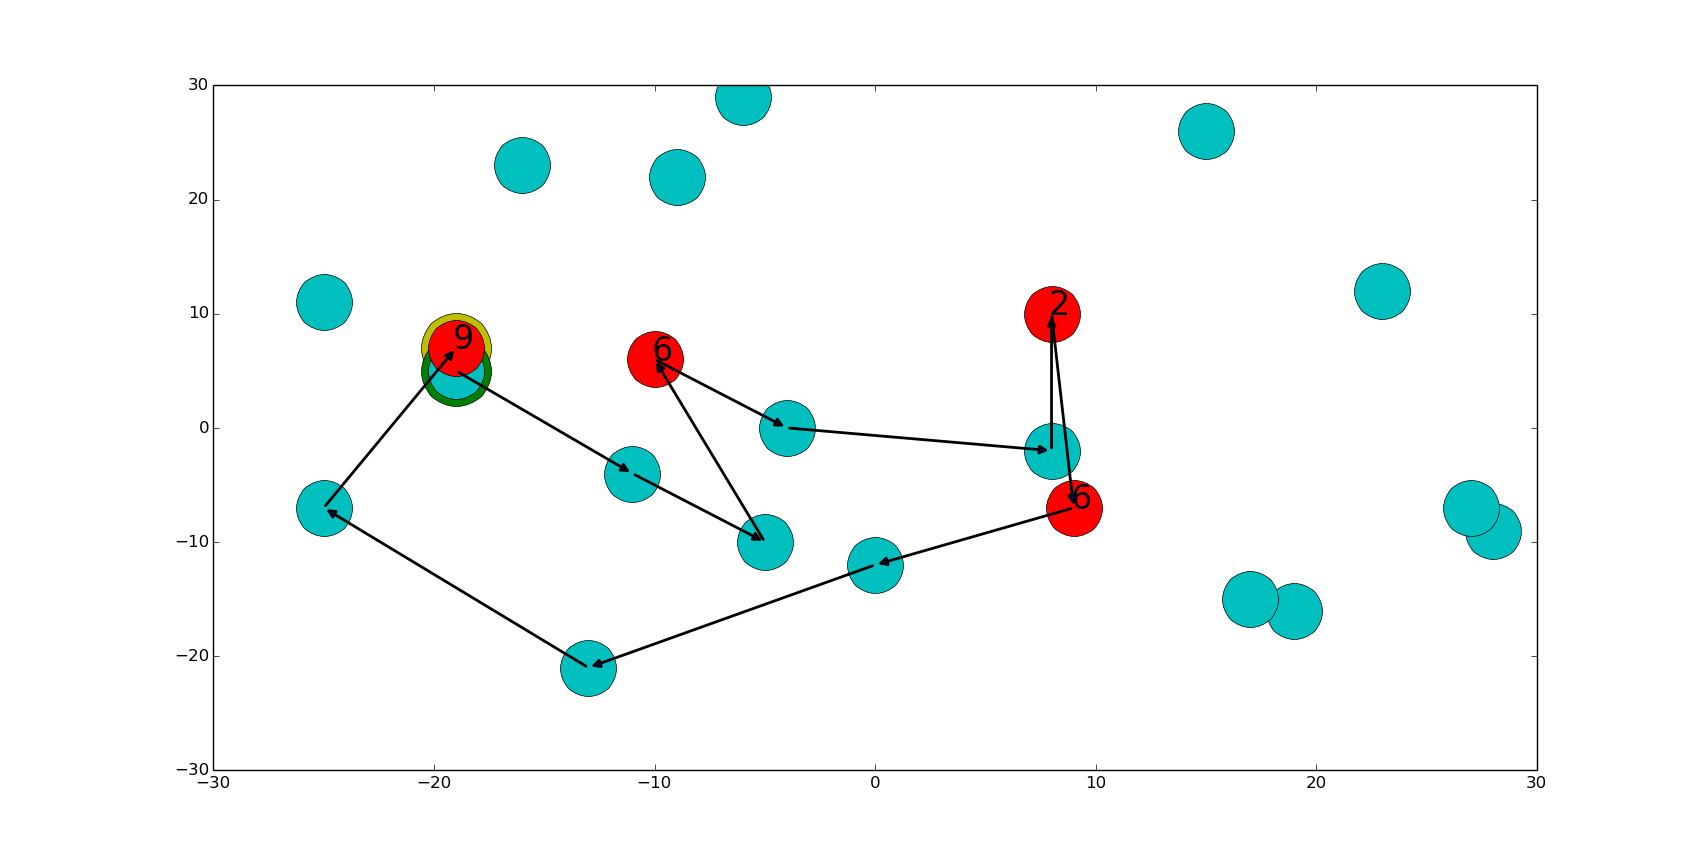
\includegraphics[scale=0.3]{./EJ5/caminoEj3opt.png}
\\{\textit{Resultado Exacto}}
  \end{center}
  \vspace*{0.3cm}

\vspace*{0.3cm} \vspace*{0.3cm}
  \begin{center}
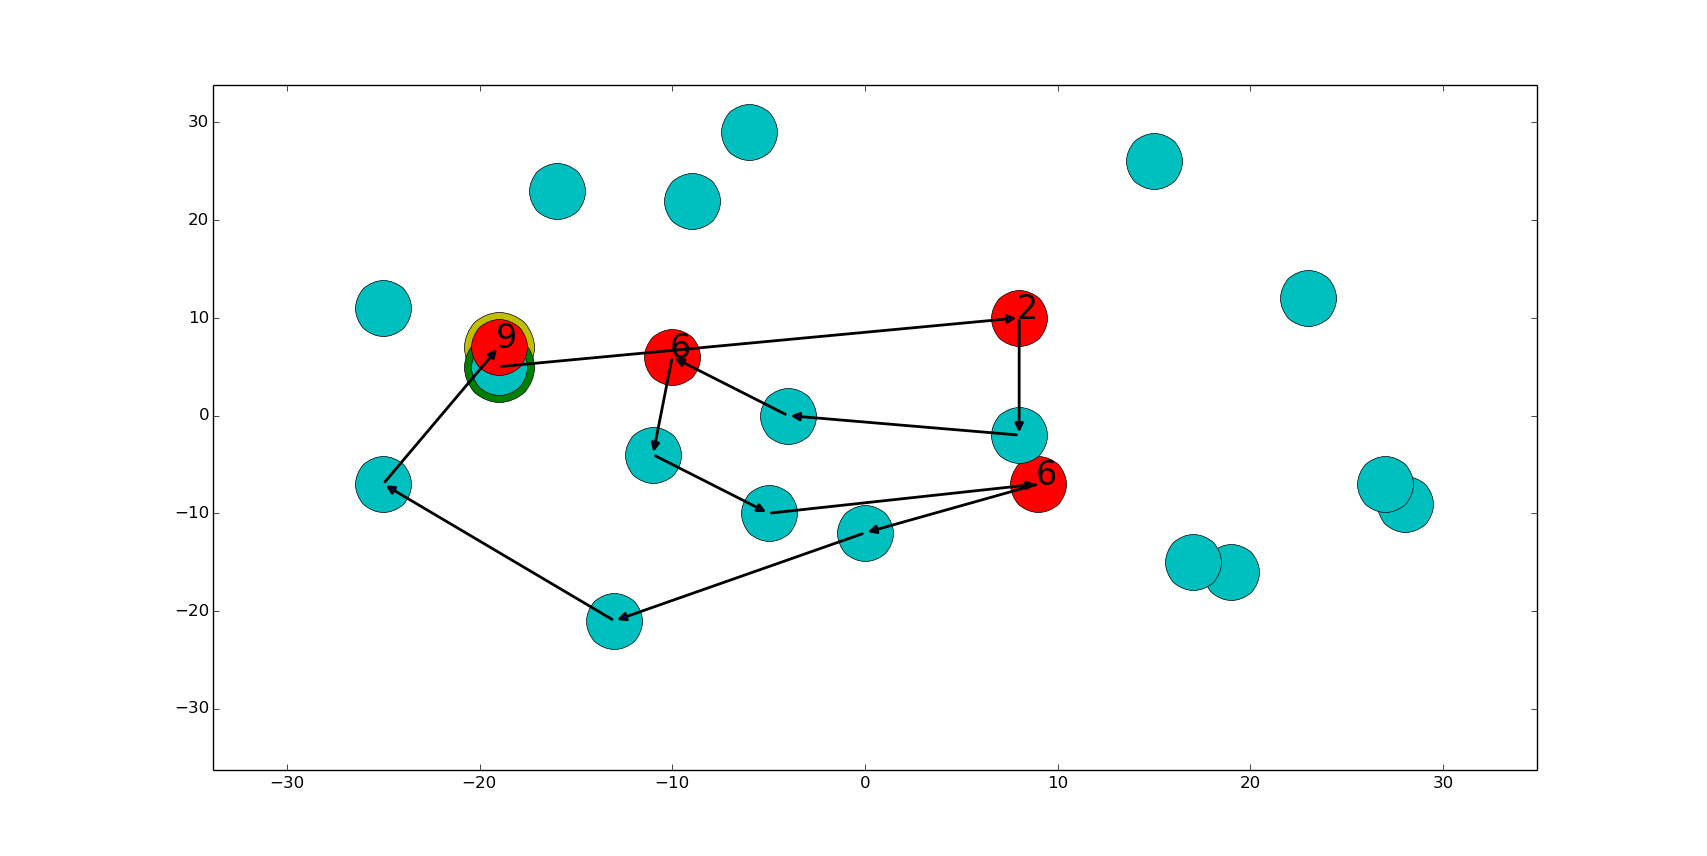
\includegraphics[scale=0.3]{./EJ5/caminoEjGoloso.png}
\\{\textit{Resultado goloso}}
  \end{center}
  \vspace*{0.3cm}
  
  \vspace*{0.3cm} \vspace*{0.3cm}
  \begin{center}
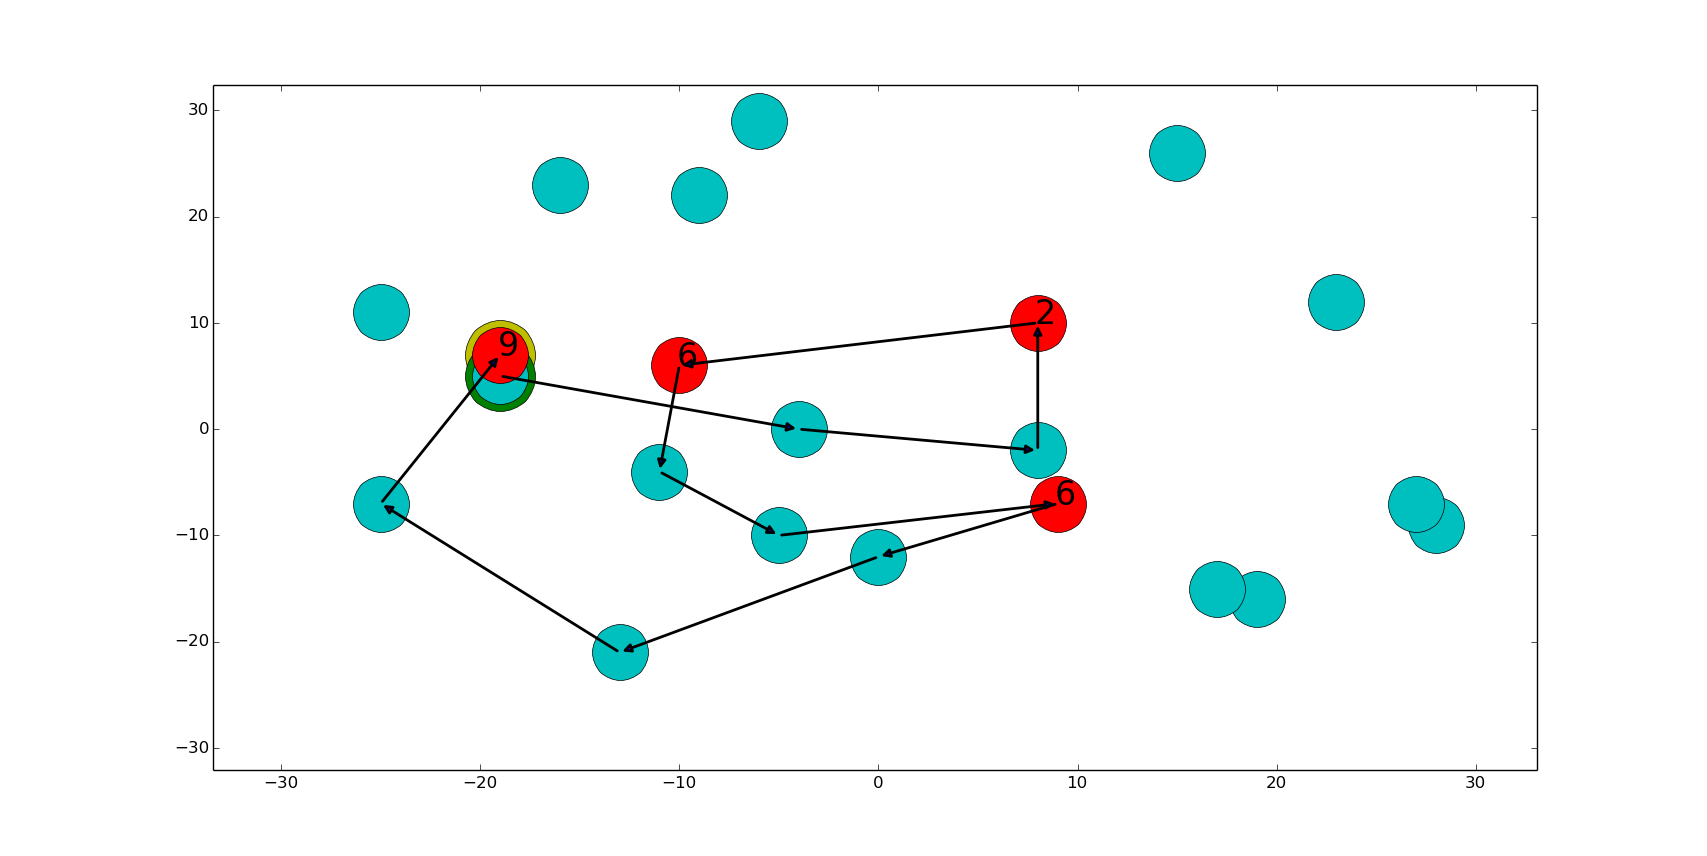
\includegraphics[scale=0.3]{./EJ5/caminoEjswap.png}
\\{\textit{Resultado SWAP}}
  \end{center}
  \vspace*{0.3cm}

  \vspace*{0.3cm} \vspace*{0.3cm}
  \begin{center}
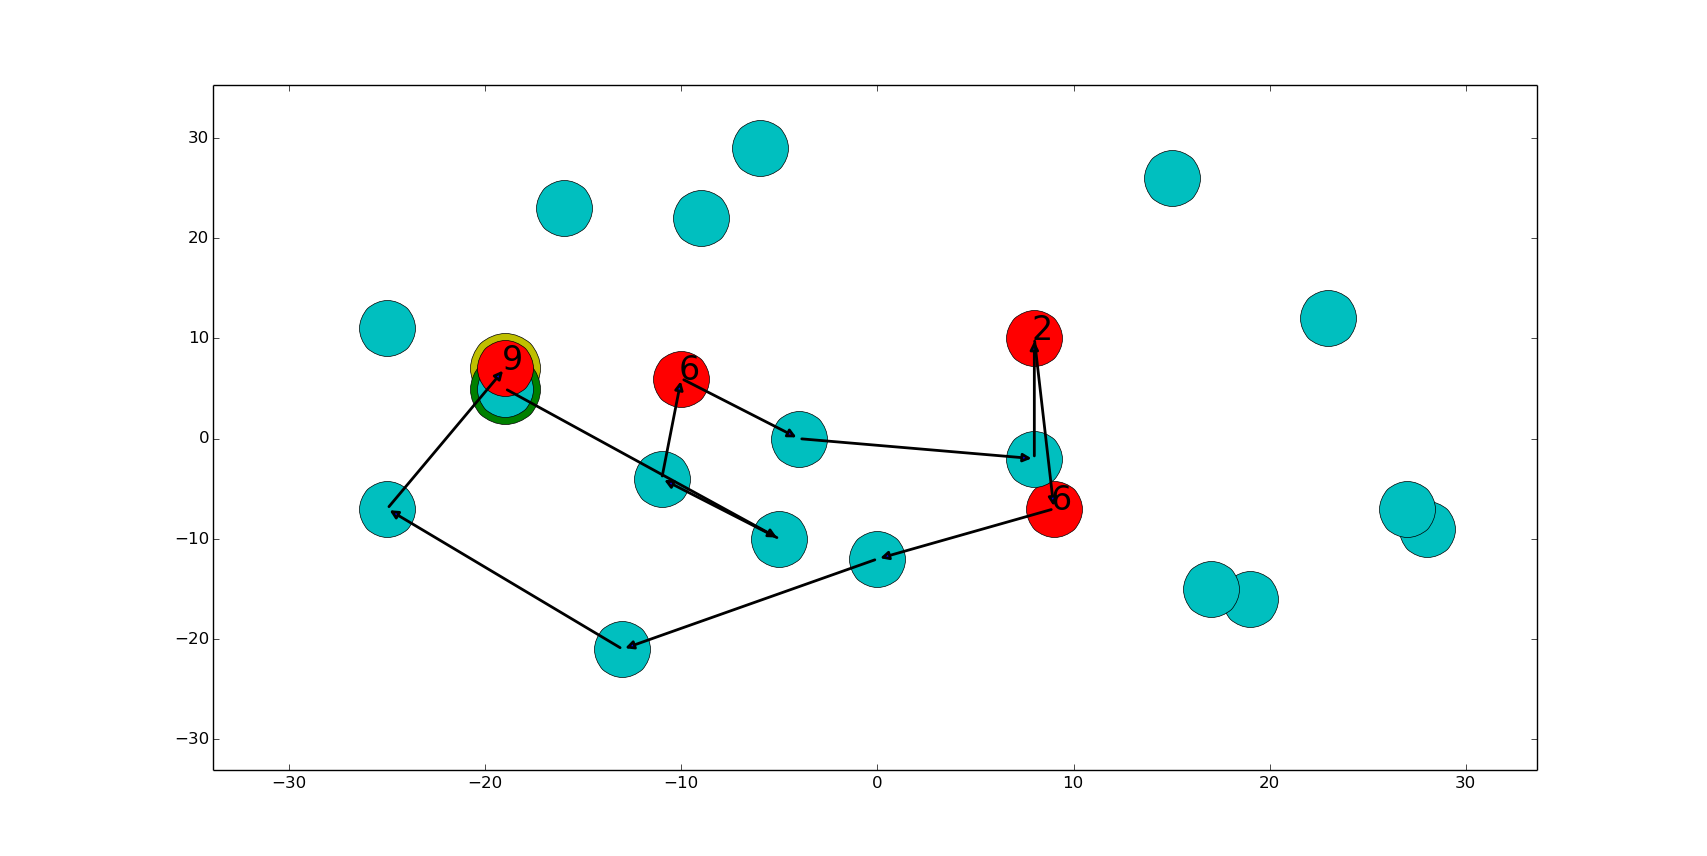
\includegraphics[scale=0.3]{./EJ5/caminoEj2opt.png}
\\{\textit{Resultado 2-OPT}}
  \end{center}
  \vspace*{0.3cm}
  
    ----> Me falta hacer
    \vspace*{0.3cm} \vspace*{0.3cm}
  \begin{center}
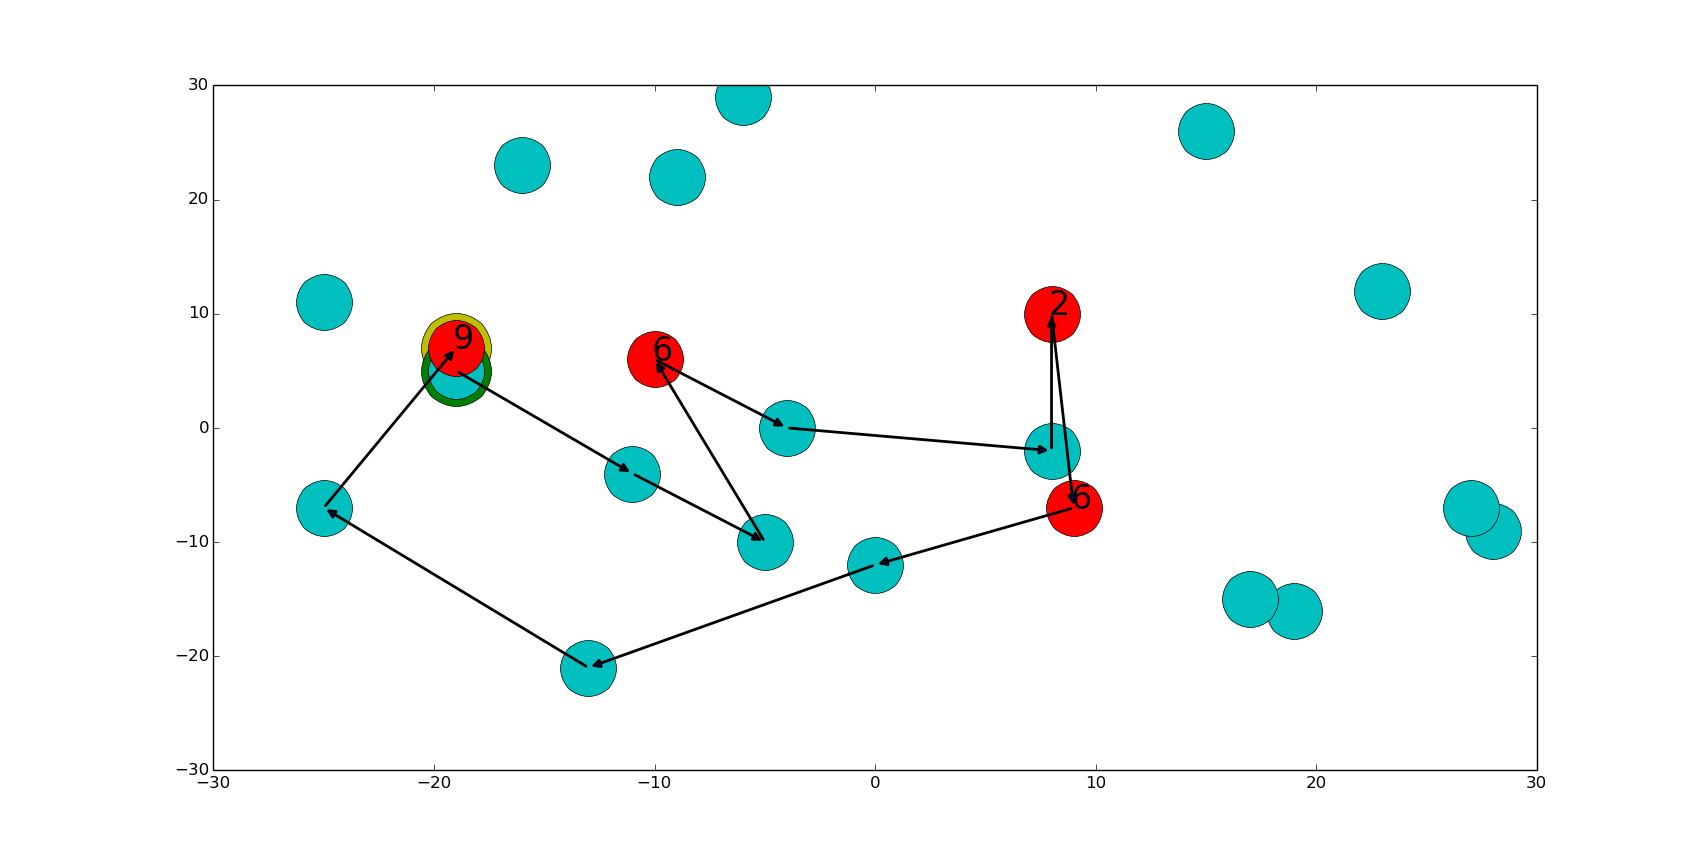
\includegraphics[scale=0.3]{./EJ5/caminoEj3opt.png}
\\{\textit{Resultado Tabu 2-OPT}}
  \end{center}
  \vspace*{0.3cm}


\subsubsection{Comparaciones de tiempo entre heuristicas}

Para corroborar la performance obtenida para este grupo de instancias se tomaron los tiempos que tarda cada algoritmo de busqueda local en obtener soluci\'on. 
 Las mediciones de las instancias de menor cantidad de elementos se compararon con la distancia exacta tomada con el backtracking. Para los casos de mayor tamaño, siendo que el tiempo de ejecución exponencial impidió la toma de mediciones, se compararon los resultados solo entre heurísticas.


\vspace*{0.3cm} \vspace*{0.3cm}
  \begin{center}
 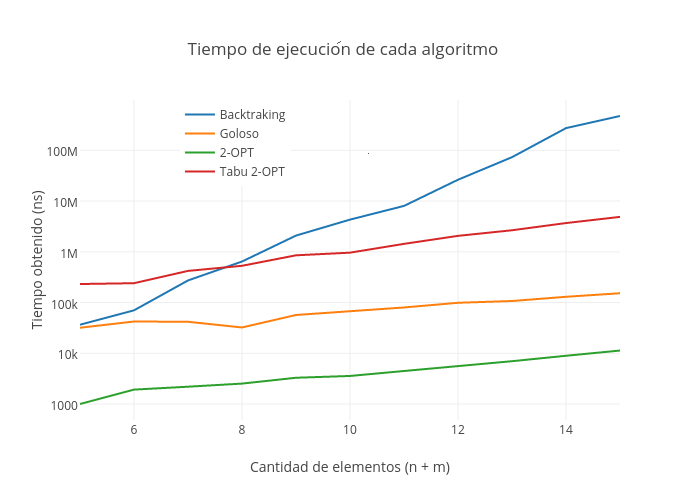
\includegraphics[scale=0.5]{./EJ5/medicionTodos.png}\\
 {\textit{Gráfico \ 5.2 - Comparaci\'on de soluciones de todos los algoritmos}}
  \end{center}
  \vspace*{0.3cm}

En una comparación de tiempo de ejecución contra el backtracking, podemos observar que el algoritmo exacto es mucho más caro en general que las aproximaciones heuristicas. Sin embargo, en el caso del Tabu search, para casos hasta 8 se ve que la solución del backtracking se logra en menor tiempo que la aproximada. No obstante, ya para casos más grandes se observa una fuerte diferenciación en los tiempos de ejecución.

\vspace*{0.3cm} \vspace*{0.3cm}
  \begin{center}
 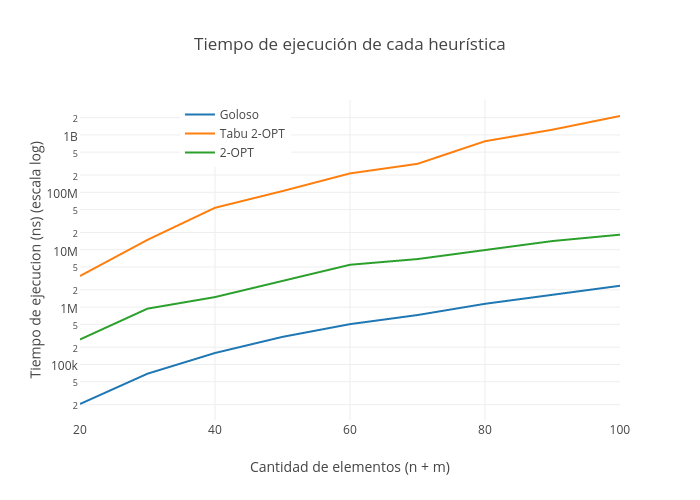
\includegraphics[scale=0.5]{./EJ5/medicion.png}\\
 {\textit{Gráfico \ 5.1 - Performance de las Heur\'isticas}}
  \end{center}
  \vspace*{0.3cm}

Dejando de lado los tiempos exponenciales del backtracking, las heuristicas comparadas ahora una frente a la otra con una mayor cantidad de instancias de diferente tamaño, permiten observar el mayor tiempo de ejecución de Tabu frente a la búsqueda 2-OPT, debido a que el primero utiliza la vecindad generada por el segundo. La referencia del algoritmo goloso nos permite dar cuenta del incremento base que tiene cada heuristica para mejorar los resultados golosos.

\subsubsection*{Calidad de solución}

Al tener en cuenta la calidad de la solución, podemos ver que la solución golosa puede diferir de la exacta enormemente, como se explico con la familia por sectores en el punto 2. Al aplicar la búsqueda local se logra disminuir esta diferencia, que luego es nuevamente disminuida al aplicar Tabu Search:

\vspace*{0.3cm} \vspace*{0.3cm}
  \begin{center}
 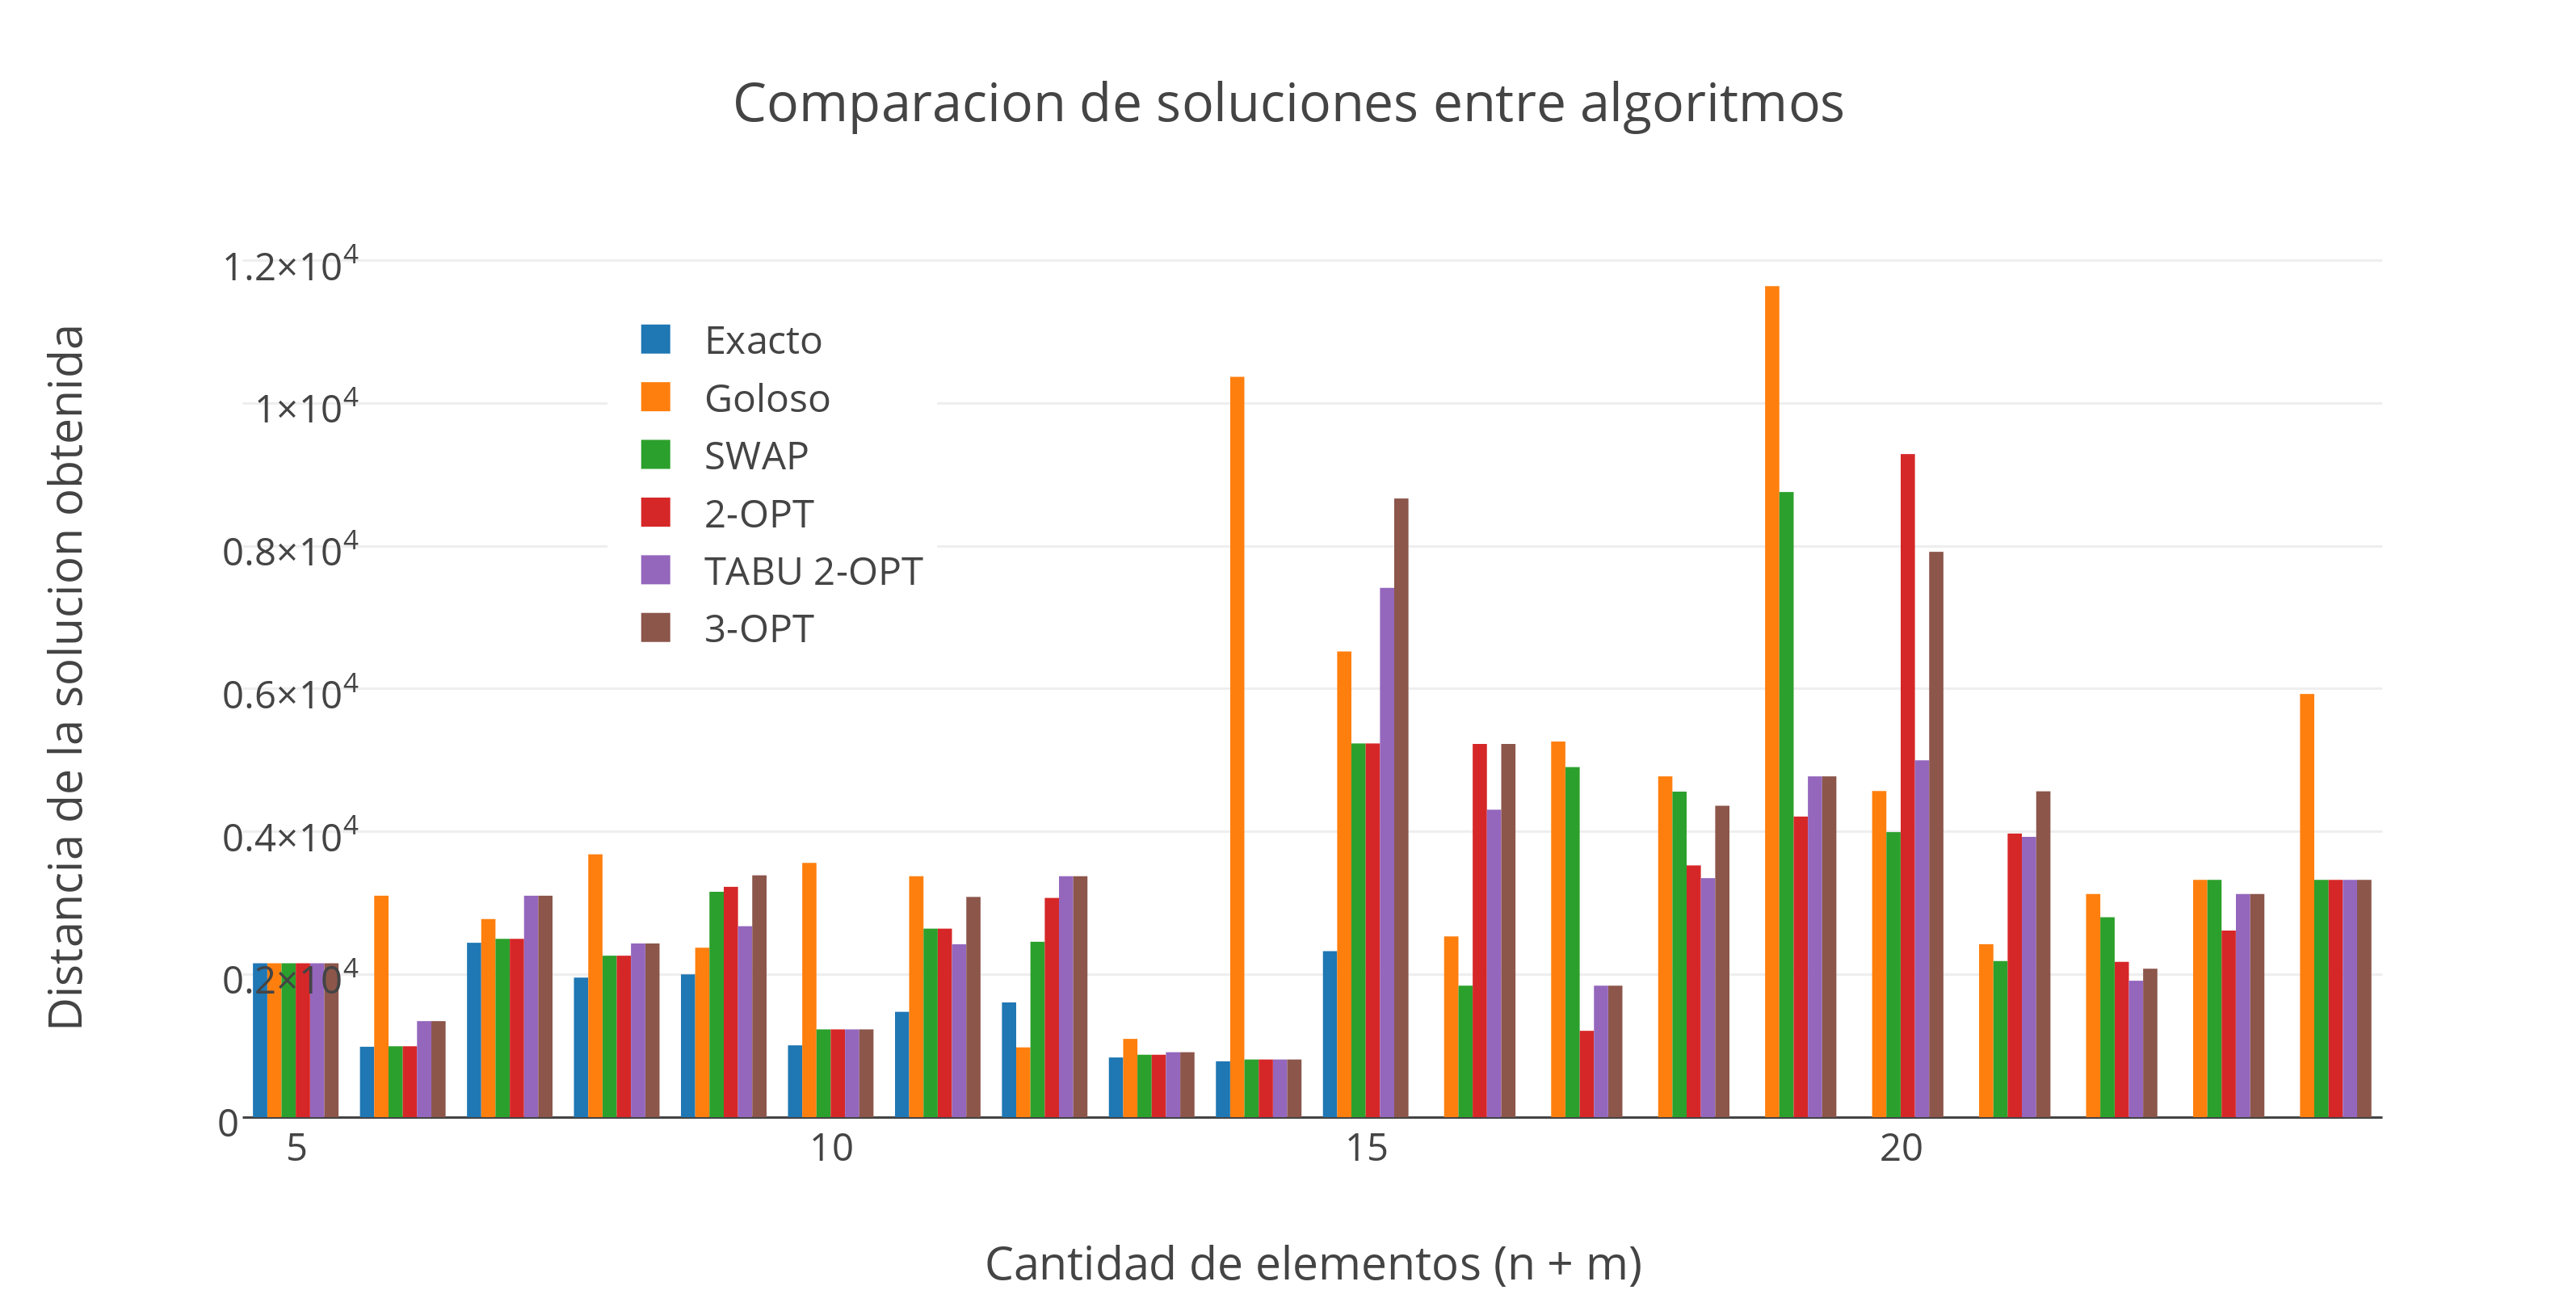
\includegraphics[scale=0.5]{./EJ5/comparativo.png}\\
 {\textit{Gráfico \ 5.2 - Comparaci\'on de soluciones de todos los algoritmos}}
  \end{center}
  \vspace*{0.3cm}
  
  \vspace*{0.3cm} \vspace*{0.3cm}
  \begin{center}
 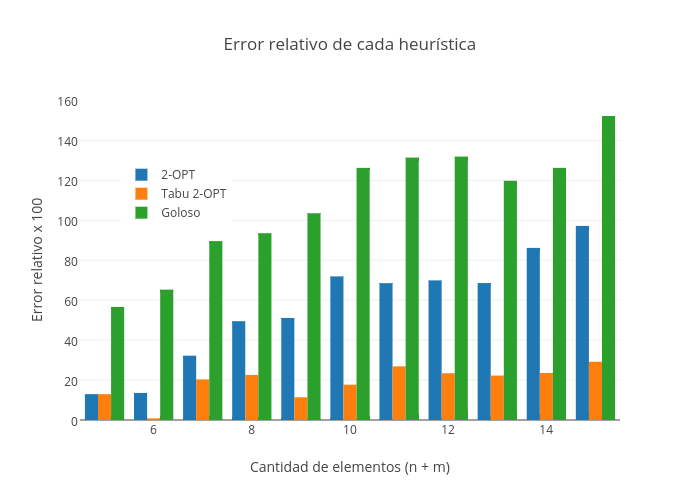
\includegraphics[scale=0.5]{./EJ5/errorChico.png}\\
 {\textit{Gráfico \ 5.2 - Comparaci\'on de soluciones de todos los algoritmos}}
  \end{center}
  \vspace*{0.3cm}

Utilizando las instancias de tamaño pequeño en donde podemos obtrener de forma exacta el resultado óptimo, podemos ver como el error de la solución golosa puede llegar a superar hasta en un $150\%$ la minima buscada. La busqueda local logra disminuír este error hasta en un $50\%$ respecto al goloso, y la aplicación de Tabú search vuelve a mejorar este error de forma que no supera el $20\%$ en diferencia con el óptimo.


\vspace*{0.3cm} \vspace*{0.3cm}
  \begin{center}
 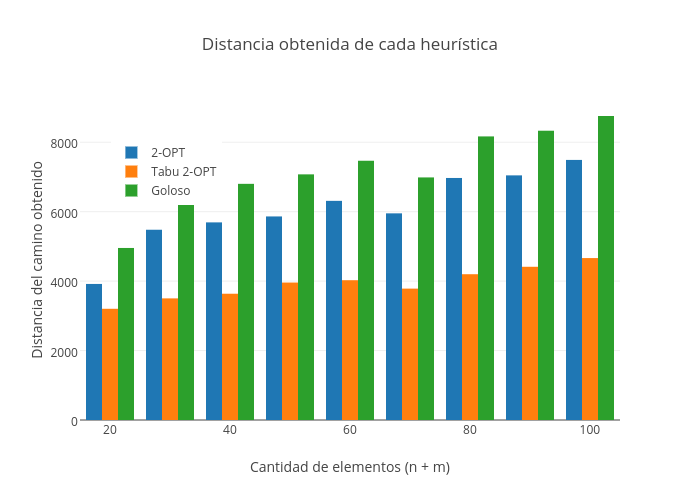
\includegraphics[scale=0.5]{./EJ5/comparativo1.png}\\
 {\textit{Gráfico \ 5.3 - Comparaci\'on de soluciones entre las heur\'isticas}}
  \end{center}
  \vspace*{0.3cm}

En una escala mayor en numero de elementos, en la cual no se cuenta con datos exactos en cuanto a solución óptima, la comparación de resultados se dará en cuenta a la menor distancia lograda posible, efectuada por cada alternativa. Como ya sucedía anteriormente, la busqueda local mejora la solución de la heuristica golosa, asi como el Tabú lo hace con el resultado de la busqueda local. La mejora de las distancias de los caminos logrados en cada conjunto de instancias de distinto tamaño es aproximadamente de un $35\%$ en cuanto a lo devuelto por Tabú frente al goloso.
%Ese ultimo porcentaje es debatible :P%

\subsubsection{Concluciones}

La resolución de ciertos problemas a nivel exacto se tornan impracticables a partir de cierto tamaño del problema a analizar, con lo cual es necesario sacrificar exactitud, por obtener al menos una solución. Al intentar solucionar este problema mediante heuristicas, se recae en el hecho de que, dado que no se tiene idea de cual es la solución buscada, es necesario obtener cierta "confianza" de las soluciones que se puedan llegar a obtener.

Al experimentar con la heuristica golosa, pudimos ver que su comportamiento lo podemos mejorar mediante la aplicacíon de busquedas locales, las cuales nos permitieron aumentar notoriamente la confianza de la solución obtenida: algunas heuristicas de busqueda, no obstante, fueron descartadas ya que  su costo/beneficio era muy alto en comparación a la del mismo méotodo goloso (Refiriendonos a 3-OPT). 

Tanto la busqueda mediante SWAP como 2-OPT nos brindaron los mejores resultados. La base de 2-OPT de Tabú nos permitio incluso mejorar lo anteriormente logrado, siendo de esta forma la metodología preferida, en cuanto a calidad de solucion. No obstante, de no contar con tanto tiempo de cómputo, la decisi\'on se deberá llevar a cabo entre SWAP y 2-OPT, las cuales se empatan bastante en calidad vs. tiempo.\\

\textbf{Experimentaciones a realizar de interés}\\
Dado que 2-OPT y SWAP obtuvieron resultados muy similares y que se implementó Tabú con el primero, es de interés desarrollar el mismo también en base a SWAP y poder realizar comparaciones entre las 2 impementaciones para poder observar su comportamierto y las diferencias que surgen entre ambos, buscando un mejor error.


\subsubsection{Dificultades afrontadas}

A lo largo del desarrollo del trabajo nos encontramos con ciertos obstaculos que tuvimos que ir sorteando:
El primero de ellos fue el tiempo necesario para correr los tests: Al manejar un algoritmo de tiempo exponencial, como es el backtraking, tuvimos que limitarnos a un pequeño grupo de instancias para obtener las mediciones exactas para las comparaciones con otros algoritmos. La utilización de la optimizacion  en la compilacion de nivel 3 (-O3) ayudo en grán medida a correr los casos más grandes y poder agrandar un poco más la muestra.\\
A la hora de tomar las mediciones de los experimentos, nos vimos con el problema de la cantidad de instancias de un mismo tamaño a tomar: siendo que no podemos tomar la misma cantidad por cada tamaño debido a que acarrea un desbalance de exactitud (las instancias más chicas tendrían más datos muestrales que las grandes), tuvimos que adaptar la muestra al n evaluado. Esto nos ocasionó un incremento substancial en la cantidad de instancias totales a evaluar, incrementando asi el tiempo de experimetación.

